\documentclass[11pt,a4paper]{article}
%\usepackage{natbib}
\usepackage[natbib=true, style=authoryear]{biblatex}
\addbibresource{citations.bib}
\usepackage[french]{babel}
\usepackage{textcomp}
\usepackage{csquotes}
\usepackage{setspace}
\usepackage{fancybox}
\usepackage{fancyhdr}
\setlength {\marginparwidth }{2cm}
\usepackage{todonotes}
\usepackage{lipsum}
\usepackage{amsmath}
\usepackage{amsfonts}
\usepackage{amssymb}
\usepackage{pifont}% http://ctan.org/pkg/pifont
\newcommand{\cmark}{\ding{51}}%
\newcommand{\xmark}{\ding{55}}%
\usepackage{bookmark}
\usepackage{mathtools}
\usepackage{scalerel}

\usepackage{diagbox, eqparbox, hhline}
% https://tex.stackexchange.com/questions/150634/how-to-force-a-text-to-appear-after-a-table
\usepackage{placeins}
\usepackage{graphicx}
\usepackage{booktabs}
\usepackage{lscape}
\graphicspath{{Img/}}
\usepackage{float}
\usepackage{titlesec}%remove chapter N
\usepackage{soul} % Texte surligné
\usepackage[left=2cm,right=2cm,top=2cm,bottom=3cm]{geometry}
\setlength{\parindent}{0cm}
\usepackage[framemethod=tikz]{mdframed} %highlight an entire paragraph
\usepackage{framed}
\usepackage{adjustbox}
\usepackage{array}
\usepackage{glossaries}


\usepackage{caption}



\usepackage{comment}


\usepackage{color,soul}
\usepackage{marginnote}
\hypersetup{
    colorlinks,
    citecolor=black,
    filecolor=black,
    linkcolor=black,
    urlcolor=blue
}

\usepackage{listings}
\lstset{
    numbers=left,
    numberstyle=\sffamily\tiny,
    escapeinside={<@}{@>}
}

\usepackage{pdfpages}

\usepackage{hyperref}

\setcounter{secnumdepth}{3}
\setcounter{tocdepth}{3}

\makeatother



\let\labelitemi\labelitemii



\setlength{\doublerulesep}{2.5pt}
\frenchbsetup{ItemLabeli=\textbullet}

\begin{document}
\newcommand{\JMUTitle}[9]{
    \thispagestyle{empty}
    \vspace*{\stretch{1}}
    {\parindent0cm
        \rule{\linewidth}{.7ex}}
    \begin{flushright}
        \vspace*{\stretch{1}}
        \bfseries\Huge
        #1\\
        \vspace*{\stretch{0.2}}
        \bfseries\Large
        #2\\
        \vspace*{\stretch{1}}
        \bfseries\large
        #4\\
        \vspace*{\stretch{1}}
        \bfseries\large
        #9
    \end{flushright}
    \rule{\linewidth}{.7ex}

    \vspace*{\stretch{1}}
    \begin{center}
        \vspace*{\stretch{1}}
        \Large #3 \\

        \vspace*{\stretch{2}}
        \large IFRES. Formasup/CAPAES\\
        \vspace*{\stretch{1}}
        \large   #8 \\[1mm]
        %\vspace*{\stretch{1}}
        \large Année académique: #5 - #6
        %large W{\"u}rzburg, den #6
    \end{center}
}
\JMUTitle
{Plan de cours : Multimédia}                                % Titel der Arbeit
{Développement de jeux vidéos dans un navigateur}                            % Muss in die Kopfzeile passen
{Plan de cours à rédiger dans le cadre du cours PESU0016}       % Art der Arbeit
{Schreurs, Daniel }                              % Vor- und Nachname des Autors
{2022}                                      % Tag der Anemeldung 
{2023}                                      % Tag der Abgabe
{Bachelor/Master Wirtschaftsinformatik}           % Studiengang
{Pascal Detroz, Dominique Verpoorten, Catherine Delfosse et Françoise Jérôme}                       % Name des Betreuers -- Hier sollte *immer* Prof. Winkelmann stehen
{Haute École de la Province de Liège}                                        % Matrikelnummer 
\clearpage
\tableofcontents
\addtocontents{toc}{\protect\thispagestyle{empty}}
\pagenumbering{gobble}



\clearpage
\pagenumbering{arabic}
\section{Informations de base}

\begin{table}[H]
    \begin{tabular}{|l|l|}
        \hline
        Cycle                                        & 1                                  \\ \hline
        Niveau du cadre francophone de certification & 6                                  \\ \hline
        Code                                         & GRA-1-048 2.2.1                    \\ \hline
        Crédits ECTS                                 & 6                                  \\ \hline
        Volume horaire (h/an)                        & 60                                 \\ \hline
        Période                                      & Quadrimestre 2                     \\ \hline
        Implantation(s)                              & TECHNIQUE - Seraing                \\ \hline
        Unité                                        & Orientation                        \\ \hline
        Responsable de la fiche                      & SCHREURS Daniel                    \\ \hline
        Pondération                                  & 60                                 \\ \hline
        Composition de l'unité d'enseignement        & Mutimédia - TP                     \\ \hline
        Prérequis                                    & /                                  \\ \hline
        Corequis                                     & (W) Développement côté client      \\ \hline
        Intervenants                                 & Maître-assistant : SCHREURS Daniel \\ \hline
        Contact                                      & {\ul daniel.schreurs@hepl.be}      \\ \hline
    \end{tabular}
\end{table}

\section{Description du cours}
Vous vous destinez à devenir des futurs techniciens du Web. Vous devez donc avoir un solide bagage qui vous permet de concevoir des contenus interactifs sur un site internet en vous servant d’un des 3 langages fondamentaux du Web... JavaScript. Dans ce cours, nous explorerons différentes techniques qui permettent d’introduire du contenus riche. Tout particulièrement en étudiant les possibilités offertes par SVG et l’API de dessin native de Canvas. Nous commencerons avec la réalisation d’animations 2D simples jusqu’à la programmation de jeux 2D plus complets. En revanche, nous n’aborderons pas les concepts 3D.
Ce cours s’inscrit dans la continuité du cours de "Développement côté client", qui a pour but de poser les bases de la programmation côté client avec JavaScript. En troisième année, dans le cadre du cours de "Développement d'applications mobiles", nous aurons régulièrement l’occasion de revenir sur certains concepts étudié dans ce cours.
\clearpage
\section{Philosophie de l’enseignant à propos de la matière du cours et/ou de l’apprentissage en général}
Mon enseignement est différencié, il vise à ce que chacun soit capable de suivre ma matière. Je fais en début de quadrimestre un test formatif afin d’avoir une vision plus précise de l’hétérogénéité de mon publique. Ainsi je peux proposer des exercices supplémentaires aux apprenants qui en auraient le plus besoin.
%(Voir Differentiated Instruction Lawrence-Brown (2004))
Le respect est au centre de mon enseignement. J’essaye d’installer un climat de confiance et de bienveillance en évitant des propos abusivement normatifs ou discriminatoires et vous encourage à faire de même.
%(Voir Andragogie)
On ne cesse d’apprendre au cours de sa vie et l’informatique est un domaine en constante évolution. J’essaye donc de répondre à cette réalité en favorisant votre autonomie. Je cherche à vous donner les clés pour comprendre les textes techniques qui vous permettront d’aborder les nouvelles technologies. Il s’agira donc beaucoup d’apprendre à apprendre. Nous aurons régulièrement l’occasion d’analyser des besoins et d’y apporter une solution concrète collectivement ou individuellement. J’utilise donc activement l’apprentissage par problèmes pour introduire les nouveaux concepts et l’apprentissage par projet pour appliquer vos connaissances. Je privilégie les activés d’apprentissage en petit groupe (moins de 20) afin de favoriser votre participation et votre sentiment d’inclusion. Je pense ainsi vous donner un cadre moins intimidant. Si je suis contraint de donner un cours en très grand groupe, je chercherai à organiser des activités variées et ludiques.
L’une de mes préoccupations est de fournir un cadre de travail qui vous motive tout en évitant la carotte et le bâton. Je tenterai de démontrer que les objectifs visés sont atteignables. Je conceptualiserai la matière afin que vous compreniez en quoi ce que je vous enseigne vous sert dans votre future profession. Le tout dans un contexte libre et autonome.

\section{Prérequis et corequis}
Ce cours de Multimédia s’inscrit dans la continuité du cours de Développement Côté Client, qui se donne au premier quadrimestre. Ce dernier vous a permis d’acquérir les bases de la programmation côté client, en JavaScript. Nous allons maintenant nous servir de ces acquis pour construire des interfaces riches. Le cours de Développement Côté Client devient ainsi le corequis du cours de Multimédia.
Si vous n’avez pas acquis les bases ou que vous éprouvez des difficultés en JavaScript, je vous encourage à refaire les exercices du cours\footnote{Je vous rappelle que les correctifs des exercices sont également disponibles depuis la branche "completed".}, regarder nos vidéos sur la chaine "\href{https://www.youtube.com/@coursdeweb}{coursdeweb}" et suivre la formation "\href{https://javascript30.com}{JavaScript30}" de \href{https://wesbos.com}{Wes Bos}.

\begin{figure}[H]
    \begin{center}
        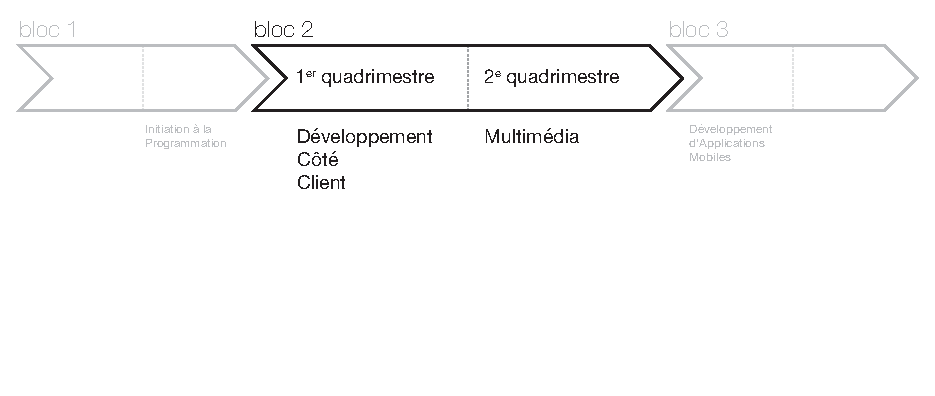
\includegraphics[width=\textwidth]{figures/corequis.eps}
        \caption{Illustration des corequis}
        \label{Fig:GQM}
    \end{center}
\end{figure}
\clearpage

\section{Contenus}
Voici dans l'ordre les différents thèmes que nous aborderons ensemble en classe :
\begin{enumerate}
    \item Le cours de (W) Multimédia
    \item Découvrir l’API SVG
    \item Animation avec SVG
    \item Utilisation d’un framework pour compiler les fichiers sources
    \item Rappel des concepts de base JavaScript utilisés dans le cadre de ce cours
    \item Découverte de l’API fetch pour récupérer de manière asynchrone des données d’une API Restful. (The Movie Database)
    \item Exercisation JavaScript. (JavaScript30 by Wes Bos)
    \item Réalisation d’un outil qui permet de générer un logo SVG à partir de paramètres encodé par l’utilisateur
    \item Introduction à l’API de Canvas
    \item Mise en place d’une boucle d’animation. Déplacer aléatoirement et à vitesse constante, des formes dans un canvas.
    \item Déplacer plusieurs cercles avec la détection du survol de la souris.
    \item Révision de quelques concepts mathématiques essentiels pour animer des cercles. (Radian, degré, périmètres, Sin, cos, etc.)
    \item Utilisez l’API Canvas pour appliquer des traitements sur des images bitmap
    \item Aborder quelques éléments de physique élémentaire. Faire tomber de la neige…
    \item Dessiner le décor d’un jeu 2D avec une sprite sheet
    \item Réalisation d’un premier jeu complet Flappybird
    \item Réalisation d’un deuxième jeu complet Asteroids
    \item Réalisation d’un examen des années précédentes
\end{enumerate}

\clearpage
\section{Visées d’apprentissage}
\begin{itemize}
    \item Utiliser efficacement l’API canvas et l’API SVG pour concevoir des contenus multimédias au sein d'un navigateur web.
    \item Réaliser\footnote{Au sens "développement" informatique.} une implémentation d’un jeux dans un navigateur web, en utilisant de manière conjointe l’API canvas, les bases du langage JavaScript et notre framework développé en classe.
\end{itemize}

\section{Méthodes d’enseignement et activités d’apprentissage}
Vous avez choisi un bachelier professionnalisant, qui cherche donc à vous préparer, au mieux, au mode professionnel. C’est donc pourquoi j’ai choisis d’articuler l’acquisition des nouveaux savoirs autour de besoins réels issus du monde professionnel. Vous aurez une fois par semaine un cours de 4 heures.
\begin{enumerate}
    \item Activités récurrentes en classe. J’alternerai ces deux activités en fonction de  la matière :
          \begin{enumerate}
              \item Développer des solutions algorithmiques, dans une forme d’autonomie individuelle ou collective, avec vos connaissances ou en allant chercher d’autres, sur base d’un problème authentique issue du monde du jeu vidéo. Par exemple, comment détecter avec JavasScript la collision de 2 formes dans un plan à 2 dimensions ?
              \item Je vous présenterai régulièrement les éclairages théoriques nécessaires à la compréhension de ces concepts algorithmiques. Parfois avant l’exercice dans quel car l’activité précède s’apparente plutôt à de l’exploration. Et d’autres fois après dans quel cas l’activité précédente s’appende plutôt à de l’exercisation.
          \end{enumerate}
    \item Activités ponctuelle vers la fin de l'année : \textit{(Activité intégrative !)}
          \begin{enumerate}
              \item Réalisation individuelle d'un examen des années précédentes. Nous consacrerons une seconde séance à sa correction collective où chacun corrige individuelle sa copie d'examen.
              \item Réalisation individuelle d'un jeu, à partir des règles. Il s’agit là d’un projet personnel que vous réaliserez à domicile en vue de vous entrainer à l’examen.
          \end{enumerate}
\end{enumerate}

\clearpage
\subsection{Justifications}
\begin{itemize}
    \item Etant donnée que la motivation fait partie de ma philosophie et que l’un des ingrédients de la motivation c’est d’apporter du sens aux connaissances l’approche intégrée me permet de rendre concret mes enseignements au travers de besoins issues de situations authentiques. Concrètement, j'articule les points de matière autours de besoins afin de faire ressentir l'interet de ces connaissances. Régulièrement quand la plupart des étudiants ont trouvé une solution, je désigne quelques étudiants pour qu’ils présentent leur solution de sorte à introduire dans un troisième temps la matière théorique (Activité 1.2). J’ambitionne ainsi de susciter leur intérêt pour la matière puisqu’ils partent de situations plutôt complexes et authentiques. Il s’agit là des deux événements dominants d’une séance de cours type.
    \item Je cherche aussi à développer l’autonomie de l’apprenant sans pour autant le submerger, avec un problème trop compliqué. Dans l’activé 1.1 le problème reste simple et abordable. En revanche pour les activités 2.1 et 2.2 l’autonomie est encore plus forte mais l’apprenant devrait à ce stade avoir acquis les compétences nécessaires. Même si la situation est nouvelle pour lui, les concepts sous-jacent restent toujours les mêmes.
    \item \cite{perrenoud1992differenciation} dit "différencier, c’est organiser les interactions et les activités de sorte que chaque élève soit constamment ou du moins très souvent confronté aux situations didactiques les plus fécondes pour lui". Autrement dit face à la diversité mathétique il faut apporter une polyvalence didactique. Et j’ambitionne aux travers de ces différents méthodes dominantes de répondre à la diversité mathétique. C’est pourquoi dans certains je laisse les étudiants explorer la documentation officiels de sorte à expérimenter les éléments dont ils ont besoin. Et d’autres fois je leur donne d’abord les éléments dont ils ont besoins et puis ils appliques la connaissance. Enfin je n'évoque pas ici tous les autres évenements
    \item "L’émission de feedbacks est souvent considérée comme un élément clé pour renforcer la motivation et soutenir la réussite des élèves."\cite{georges2011feedbacks}. La réalisation de l'examen ainsi que le projet personnel (activités 2.1 et 2.2), sont 2 occasions pour l'étudiant de recevoir du feedback. D'une part sur sa la comprension de la matiière, donc plutot un feedback simple de type assertif et évaluatif \cite{georges2011feedbacks} sur la performance. D'autre part un feedback plus complexes relatif aux startégies qu'il faut adapaté. Quel sont les parties plutot simples et comment rapidement les validés. Ou encore réfléchir aux éléments plus compliqué, que mes étudiants aiment appeler des "pièges"\footnote{Je n'adère évidement pas à cette appélation. Mon examen ne contient pas de piège sans quoi on pourrait se poser des questions sur mes intentions. L'examen contient des parties plus compliqué qui nécessitent une certaine forme d'inibition cognitive.}. De plus \citep{hattie2008visible} explique dans son ouvrage que le feedback a un impact significatfif sur la performance de l'étudiant. Enfin c'est une occasion pour entrainer la méta-cognission\cite{leclercq2008modele}. Nous réfléchisson ensembre aux startégies qu'il faut mettre en place pour réusir l'examen. D'ailleurs chaque année je désigne un "sécrétaire" qui devra prendre notes de toutes les astuces que nous avons déterminé ensemble afin que les étudiants puisse consulter cette resource plus tard.
\end{itemize}



\clearpage
\printbibliography

\end{document}
